\section{Research methodology}
The development process from Heath et al.~\cite{heath2009survey}, see figure~\ref{fig:steps_simulation},  will be followed.

The process consists of several rounds.
All steps below where conducted in a loop.
Later rounds influenced earlier rounds.

\paragraph{Formulating the problem and objectives}
The formulation of the problem and objectives is already complete, they are mentioned as the research goals in the previous section.

\paragraph{Conceptional validation}
The second round consists of building and validating the conceptual model.
%It relies upon known system theories, drives model development and dictates the variety of assumptions required in any model abstraction process.

The importance of the conceptional model is mentioned by Heath et al.~\cite{heath2009survey}: the conceptual model forms the foundation of an ABM model; an invalid conceptual model indicates the model may not be an appropriate representation of reality.

Therefore, in this round the abstraction level will be determined.
The model based approach is a way to eliminate all variables not direct related to the problem and keep only the essence of the situation.
The model must, in a highly abstracted way, still mimic some real behavior and real world elements

The conceptional model consists of:\\
-which agents exist along with their behavior rules,\\
-a representation of the world with roads, building and their rules.\\

All other interesting variables must be defined, such as simulation period, number of agents of each type, can agents leave and if so when.

\paragraph{Translate into computer model}
This round converted the conceptional model into computer code.

As mentioned, the multi-agent programmable modeling environment used in this study was NetLogo~\footnote{\url{ccl.northwestern.edu/netlogo/}}.

This environment and programming language needed some studying, for this: the NetLogo online user manuals~\footnote{\url{ccl.northwestern.edu/netlogo/docs/}} and other existing models where used.

A large part of the world is bases on an existing model,i.e., the Taxi Cab model~\cite{dongpingtaxicabs2019} see: figure~\ref{fig:taxicabmodel}.

\begin{figure}
    \centering
    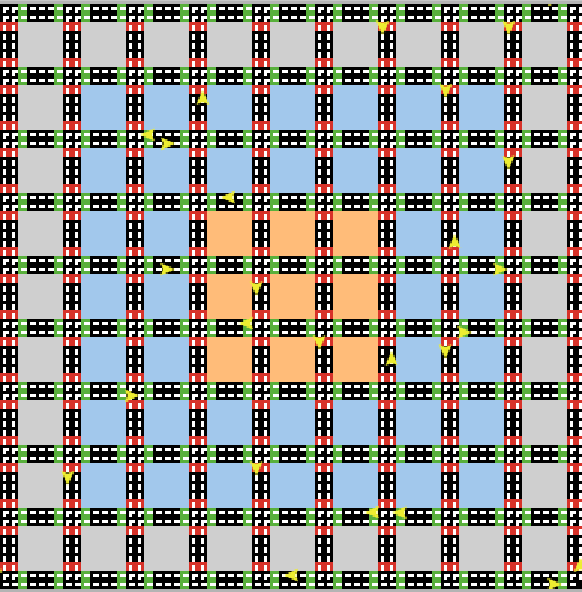
\includegraphics[width=8cm]{sections/pics/Taxi Cabs}
    \caption{Taxi Cab Model}
    \label{fig:taxicabmodel}
\end{figure}

\paragraph{Run simulations and obtain results}
With the ready model, simulations were run.
To automate the simulation and setting some variables, a Python package called pyNetLogo~\footnote{\url{pynetlogo.readthedocs.io/}} was used.
This package can start a NetLogo program, set some variables and run it for some given time.
The results then can be retrieved and be used to make diagrams.
This way enables running many simulations and automate making the diagrams.










